\documentclass[8pt]{beamer}
\usetheme{Dresden}

\usepackage[latin5]{inputenc}
\usepackage[english]{babel}
\usepackage{amsmath}
\usepackage{amsfonts}
\usepackage{amssymb}
\usepackage{graphicx}
\usepackage{subcaption}
%\usepackage{subfig} 
\usepackage{algorithm} 
\usepackage{algorithmic}

\title{A Distributed Greedy Heuristic for Computing Voronoi Tessellations With Applications Towards Peer-to-Peer Networks}
\author{Brendan Benshoof \qquad Andrew Rosen \qquad \\Anu G. Bourgeois \qquad Robert W. Harrison \\Department of Computer Science, Georgia State University}
%\subtitle{}
%\logo{}
%\institute{}
%\date{}
%\subject{}
%\setbeamercovered{transparent}
%\setbeamertemplate{navigation symbols}{}

\begin{document}
	\maketitle
	
	
	
\begin{frame}{Outline}
	\tableofcontents
\end{frame}
	
	
\section{Background}
\subsection{Motivation}
	
	\begin{frame}{Motivation}
		We were creating a distributed network based off of Delaunay Triangulation and needed a fast distributed algorithm for calculating Delaunay peers.
		We ran into a couple of issues.
		\begin{itemize}
			\item Distributed algorithms for solving Delaunay triangulation don't really exist (every node does a global solution).
			\item Not any fast solutions if we start moving out of 2D Euclidean space.
		\end{itemize}
		This leaves approximation.  However:
		\begin{itemize}
			\item Simple approximation doesn't guarantee a fully-reachable network ($k$-nearest neighbor, nodes in radius $r$).
			\item Other solutions \cite{voronet} required prohibitively high sampling or other hidden time costs.
		\end{itemize}
		And nothing can handle moving nodes.
	\end{frame}		
	
	
	
	

		
		
		
		
		
	
	\subsection{Distributed Hash Tables}
	\begin{frame}{Distributed Hash Tables}
		\begin{itemize}
			\item Abstractly, a DHT is a mechanism for maintaining a large state in a decentralized network.
			\item In practice, the state is a large number of $ (key, value) $ records.
			\item A Distributed hash table assigns those records to servers and routes request for those records to those servers.
			\item Current incarnations of Distributed hash tables assign servers and records locations in an arbitrary metric space.
			\item Servers are assigned responsibility for records that are ``close'' to them, and to peer with ``nearby'' servers.
			\item DHTs currently use a variety metric spaces.
		\end{itemize}


	\end{frame}

	\begin{frame}{Applications of DHTs}
		\begin{itemize}
			\item \textit{P2P file sharing} is by far the most prominent use of DHTs.  
			The most well-known application is BitTorrent \cite{bittorrent}.
			\item \textit{Distributed Domain Name Systems} (DNS) have been built upon DHTs \cite{cox2002serving} \cite{pappas2006comparative}.
			Distributed DNSs are much more robust that DNS to orchestrated attacks, but otherwise require more overhead.
			%\item Distributed search (faroo)
			\item Distributed \textit{machine learning} \cite{liparameter}.
			\item Many \textit{botnets} are now P2P based and built using well established DHTs \cite{saad2011detecting}. 
			This is because the decentralized nature of P2P systems means there's no single vulnerable location in the botnet.
		\end{itemize}
	\end{frame}

\begin{frame}{Extant Varieties of DHT}
	\begin{itemize}
		\item Ring Based DHTs
		\begin{itemize}
			\item Chord
			\item Pastry
			\item Tapestry
		\end{itemize}
		\item Tree Based DHTs
		\begin{itemize}
			\item CAN
			\item Kademlia
		\end{itemize}
	\end{itemize}
\end{frame}

\begin{frame}{How are DHTs and Vonroi Tesselation/Delunay Trianguation related?}
	A Server is responsible for records ''close`` to it (Voronoi Triangulation)
	A Server peers with other servers that bound it's Voronoi Region (Delunay Triangulation)
	DHTs often have peers in excess of the Delaunay triangulation to shorten lookups, however the peers that are the Delunay neighbors
	\begin{itemize}
		\item Ring Based DHTs
		\begin{itemize}
			\item Chord: a unidirectional modulus ring metric
			\item Pastry, Symphony: bidirectional modulus ring
		\end{itemize}
		\item Tree Based DHTs
		\begin{itemize}
			\item CAN: Euclidean distance
			\item Kademlia: XOR distance
		\end{itemize}
	\end{itemize}
\end{frame}


\begin{frame}{Why do we need DGVH?}
	\begin{itemize}
		\item The different topologies DHTs utilize present optimization trade-offs (lookup latency, number of lookup hops, network robustness, availability, processing overhead)
		\item The primary effort in implementing a new metric space in a DHT is implementing Voronoi Regions/Delunay Triangulation algorithm in that metric.
		\item DGVH allows many metrics to be tested without requiring the design and development effort of generating an exact Voronoi Regions/Delunay Triangulation algorithm.
		
	\end{itemize}
\end{frame}



	

	
\section{DGVH}
	\begin{frame}{Distributed Greedy Voronoi Heuristic}
		\begin{itemize}
			\item Geometrically intuitive method of approximating the one-hop delaunay peers of a Node
			\item Is guaranteed to form a connected mesh (unlike k-nearest heuristic)
			\item Can be utilized in any continuous metric space
		\end{itemize}
		
	\end{frame}
	
	\subsection{Our Heuristic}
	
	
	\begin{frame}{DGVH Algorithim}

			\begin{algorithmic}[1]  % the numberis how many lines
				\STATE Given node $n$ and its list of $candidates$.
				\STATE $peers \leftarrow$ empty set that will contain $n$'s one-hop peers
				\STATE Sort $candidates$ in ascending order by each node's distance to $n$
				\STATE Remove the first member of $candidates$ and add it to $peers$
				\FORALL{$c$ in $candidates$}
				\STATE $m$ is the midpoint between $n$ and $c$
				\IF{Any node in $peers$ is closer to $m$ than $n$}
				\STATE Reject $c$ as a peer
				\ELSE
				\STATE Remove $c$ from $candidates$
				\STATE Add $c$ to $peers$
				\ENDIF
				\ENDFOR
			\end{algorithmic}

	\end{frame}
	
	
	
\begin{frame}{Visual Intutution}
	PUT PICTURES HERE!!!!
\end{frame}
	
	
	
	
\subsection{Peer Management}
	\begin{frame}{Realistic Candidate set Size}
		\begin{itemize}
			\item In application, a single node will not need to calculate the triangulation for every peer in the network, rather it will only calculate it's own peers.
			\item A smart ''join`` process will prevent the Candidate Set from reaching $O(n)$
			\item Expected size of the candidate set is $O(degree^2)$ which compromises current peers and 2-hop peers
			\item The average degree of many metric spaces is $O(1)$, then therefore DGVH will practically run in $O(1)$ time in those metric spaces.
		\end{itemize}
	\end{frame}
	\begin{frame}{Error Mitigation}
		\begin{itemize}
			\item As DGVH is a heuristic, it will likely have errors when compared to a global Delaunay triangulation.
			\item This error rate is difficult to find analytically and will vary between metric spaces and distributions of locations
			\item A simple method of mitigating this error is to keep both one and two hop peers.
		\end{itemize}
	\end{frame}
	
\subsection{Algorithm Analysis}
	
	
\section{Experiments}
	
\subsection{Heuristic Accuracy}


\begin{frame}{Results}
\begin{figure}
	\centering
	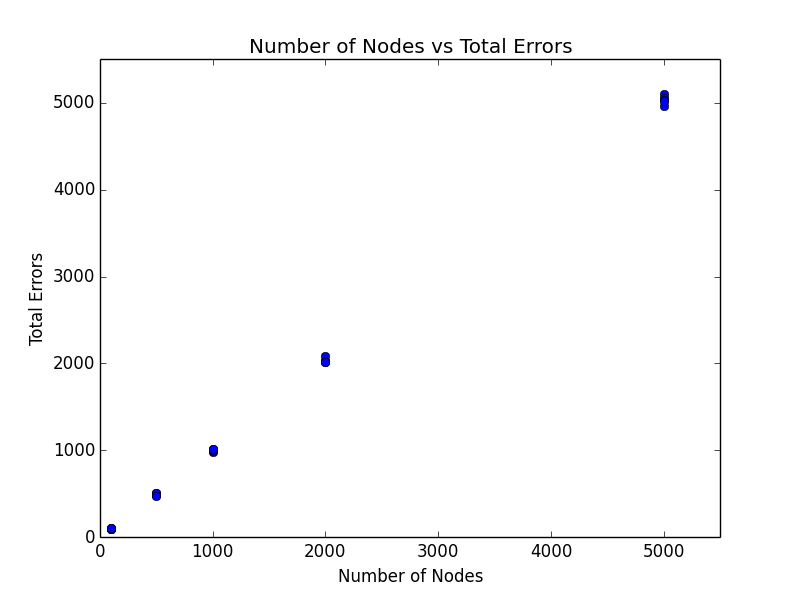
\includegraphics[width=0.5\linewidth]{error_rate}
	\caption{As the size of the graph increases, we see approximately 1 error per node.}
	\label{exp_0}
\end{figure}
\end{frame}

\subsection{Routing Accuracy}
\begin{frame}{Results}
 \begin{figure}
 	\label{fig:conv}
 	\centering 
 	\begin{tabular}{cc}
 		
 		\begin{subfigure}{\columnwidth}
 			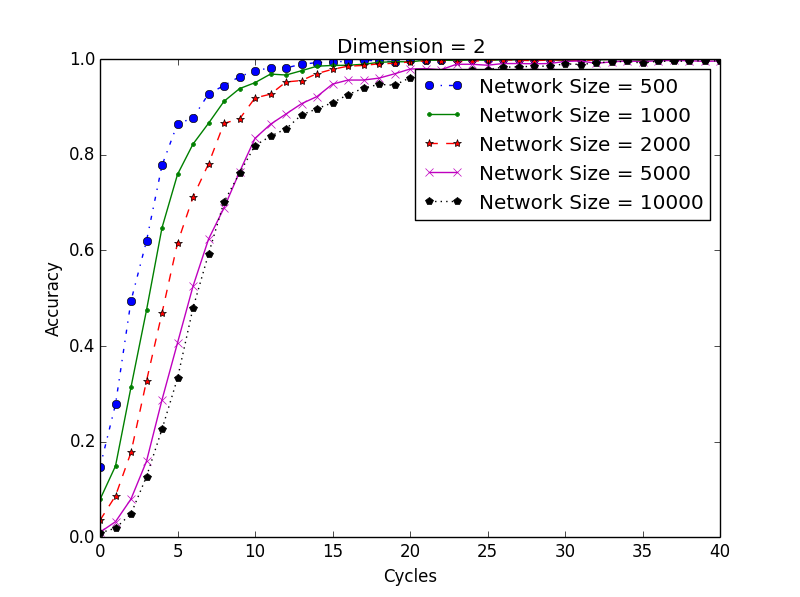
\includegraphics[width=\columnwidth]{conv_d2}
 			\caption{This plot shows the accuracy rate of lookups on a 2-dimensional network as it self-organizes.}
 			\label{conv2}
 		\end{subfigure} &
 		
 		\begin{subfigure}{\columnwidth}
 			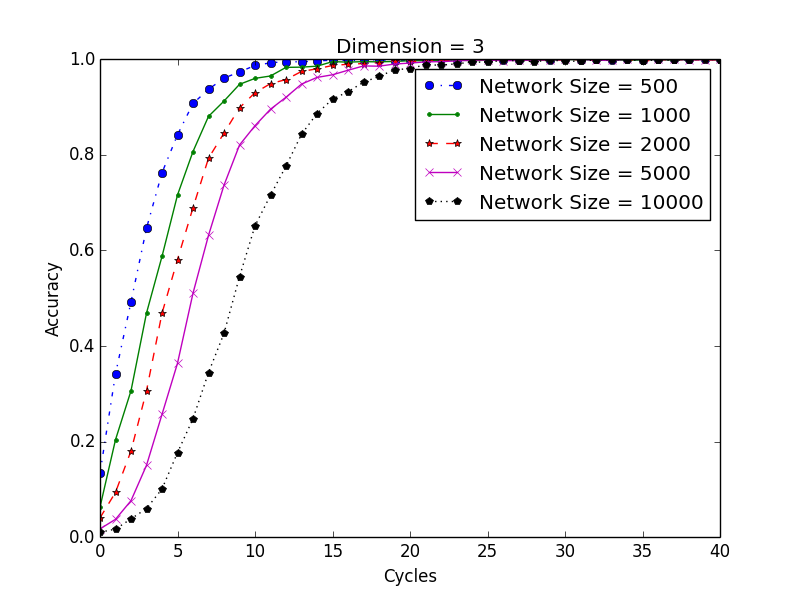
\includegraphics[width=\columnwidth]{conv_d3}
 			\caption{This plot shows the accuracy rate of lookups on a 3-dimensional network as it self-organizes.}
 			\label{conv3}
 		\end{subfigure} \\
 		
 		\begin{subfigure}{\columnwidth}
 			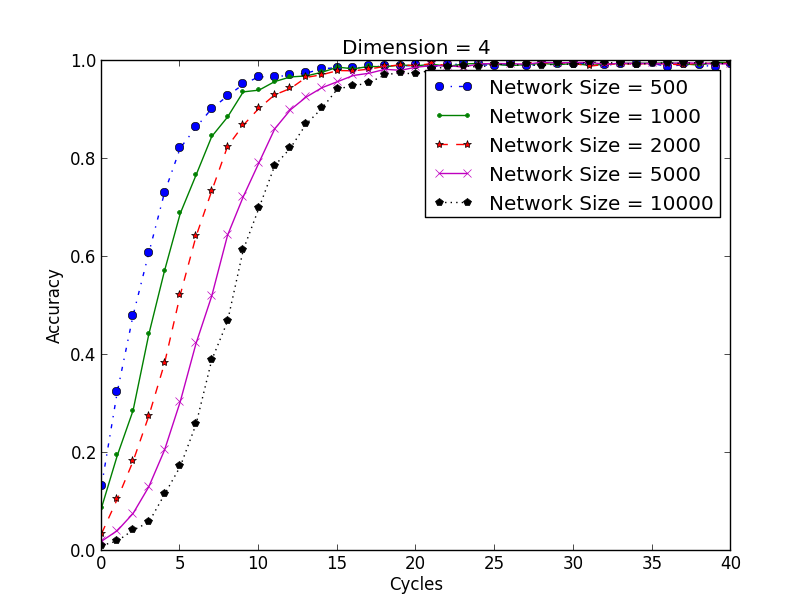
\includegraphics[width=\linewidth]{conv_d4}
 			\caption{This plot shows the accuracy rate of lookups on a 4-dimensional network as it self-organizes.}
 			\label{conv4}
 		\end{subfigure} &
 		
 		
 		\begin{subfigure}{\columnwidth}
 			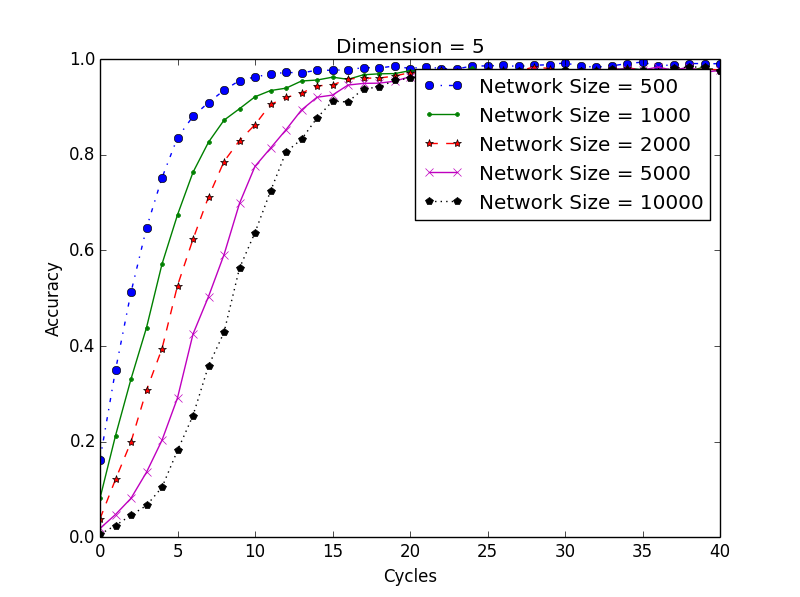
\includegraphics[width=\linewidth]{conv_d5}
 			\caption{This plot shows the accuracy rate of lookups on a 5-dimensional network as it self-organizes.}
 			\label{conv5}
 		\end{subfigure}
 		
 	\end{tabular}
 	\caption{These figures show that, starting from a randomized network, DGVH forms a stable and consistent network topology.
 		The Y axis shows the success rate of lookups and the X axis show the number of gossips that have occurred.
 		Each point shows the fraction of 2000 lookups that successfully found the correct destination.}
 	
 \end{figure}

	
	


\end{frame}	

\section{Conclusion}
	\begin{frame}{Other Applications}
		One type of distributed system that can use Voronoi tessellations are \textit{wireless ad-hoc networks}.
		\begin{itemize}
			\item Solves the coverage-boundary problem \cite{carbunar2004distributed}.
			\item Can be used for sleep scheduling \cite{chen2008voronoi}
		\end{itemize}
	\end{frame}	
	

\bibliography{P3DNS}
\bibliographystyle{plain}
	
\end{document}